\documentclass[a4paper,10pt]{article}
\usepackage{caption}
\usepackage{cite}
\usepackage{pythonhighlight}
\usepackage{graphicx, subfigure}
\usepackage{hyperref}
\usepackage[english]{babel}
\usepackage[latin1]{inputenc}
%
\begin{document}
\captionsetup[figure]{labelfont={bf},name={Fig},labelsep=period}
%
   \title{Mystic Kernel Size in CNN}

   \author{Lei Shiye}
          
   \date{2019\\ March}

   \maketitle
 
  \newpage
    
% This is a comment: in LaTeX everything that in a line comes
% after a "%" symbol is treated as comment
\hypersetup{colorlinks=true, bookmarks, unicode}
\section*{Abstract}
% When adding * to \section, \subsection, etc... LaTeX will not assign
% a number to the section
With the fast development in deep learning filed, there are more and more deep 
neural networks(\textbf{DNN}) with various architectures. Besides, the number of 
layers in DNN is becoming larger and larger. Under the circumstance, some features 
between basic convolutional neural network(\textbf{CNN}) may be overlooked by us, 
like kernel size. In this report, I focus on the how the size of kernel in CNN have
a influence on deep learning process. Through testing a same CNN with different 
kernel size on different dataset, we can find some interest phenomenons and extract
some information from them. 


\paragraph{Note:}
The source codes ralated to the report can be found on github:
\begin{verbatim} 
      https://github.com/LeavesLei/UPC-DL-lab-code
\end{verbatim}

\section{Introduction}

\paragragh After AlexNet\cite{NIPS2012_4824} showing strong strength in ImageNet competition in 2012, deep learning
has received the attention of many people. In a basic image classification task, a DNN with some 
convolutional layers, pooling layers and full connected layers is used to extract information from 
image dataset. We often devide the image dataset into two subset: training dataset and validation 
dataset during training process. Maybe we could do the dataset augmentation before put them into 
network. After some epochs, we can get DNN weights for the classification task.


At the same time, neural networks became deeper and deeper and the final accuracy is
 higher and higher. But the most critical part of DNN is still convolutional layer.
Lots of beginners including me in the filed of deep learning is a little hard to 
understand that why the small convolutional kernel could extract huge information from 
image. 
 

So I decided to do some reseach about convolutional kernel size. More specifically,
I want to figure out whether there is a relationship between convolution kernel size and 
final accuracy in an image classification task. 
 
 
\section{Methods}
To focus on convolutional kernel size, I didn't use DNN with complex architecture like VGGNet\cite{simonyan2014very} or 
ResNet\cite{he2016deep} but LeNet-5\cite{lecun1998gradient}, a classic CNN. The architecture of LeNet is presented in Fig ~\ref{Fig.LeNet-5}

\begin{figure}[htpb]
\centering 
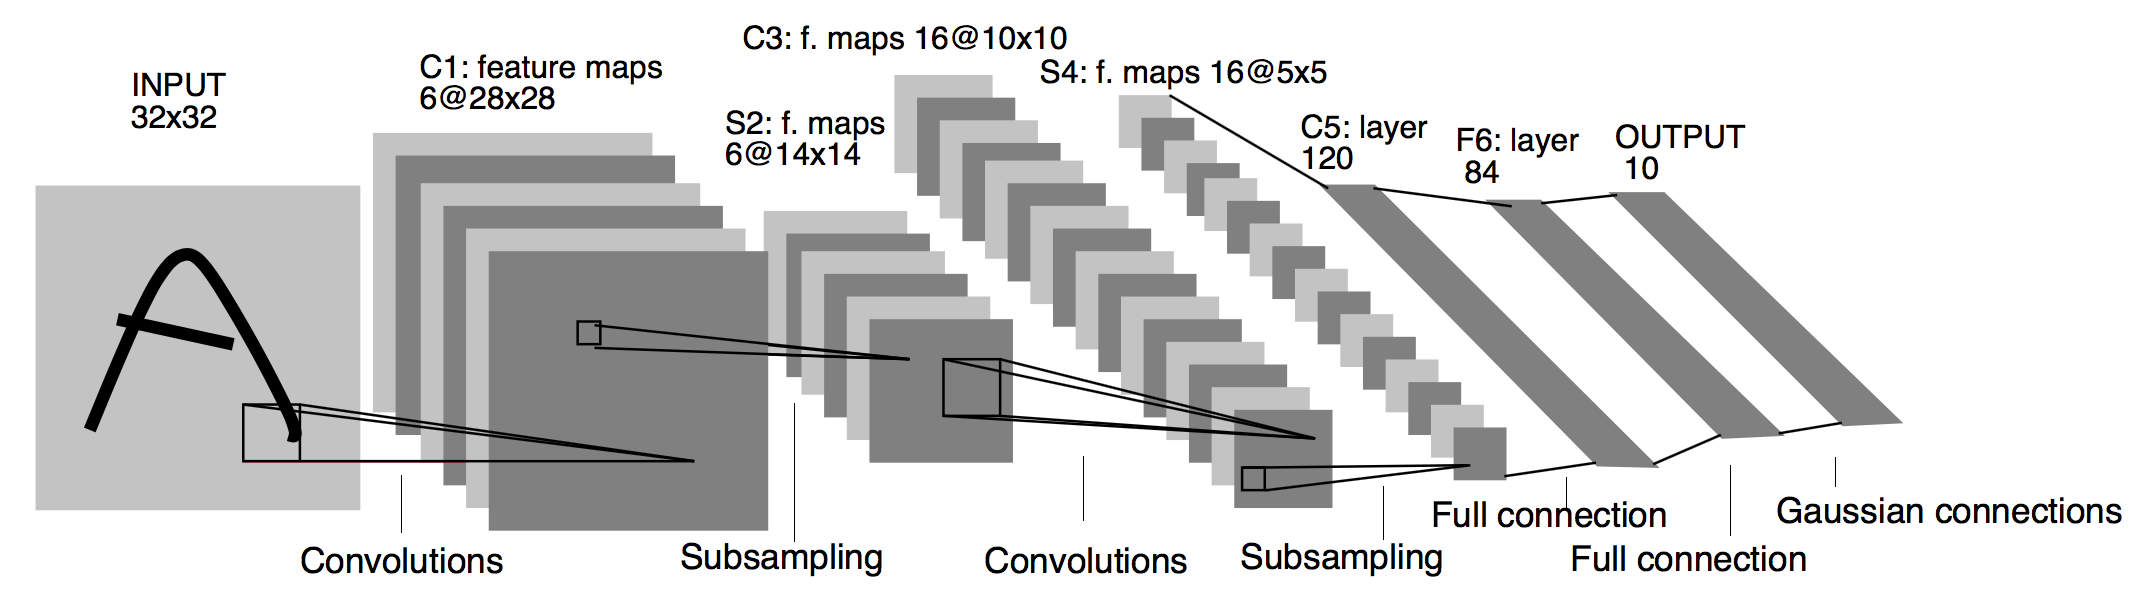
\includegraphics[width=1\textwidth]{report_image/LeNet5.png} 
\caption{LeNet-5} 
\label{Fig.LeNet-5} 
\end{figure}

\subsection{CNN architecture}
LeNet-5 is often used to deal with MNIST whose figure size is $28\times28$. In this report, I used 
several image datasets which image sizes is far greater than MNIST. So the CNN should have a greater
amount of weight than basic LeNet-5. So I changed some details based LeNet-5. The specific structure
of the CNN used in the report is as follows:

   \begin{enumerate}
      \item  C1: is a convolution layer with 32 filters.
      \item  S2: is a max pooling layer with a $2\times2$ kernel size.
      \item  C3: is a convolution layer with 62 filters
      \item  S4: is a max pooling layer with a $2\times2$ kernel size
      \item  F5: is a full connected layer with 500 units.
      \item  Output layer: the number of unit is same as dataset classes.
  \end{enumerate}
 
I used Python with Keras library in the report. The codes of building CNN are as follow:

\begin{python}
 model = Sequential()
    model.add(Conv2D(32, kernel_size=(kernel_size, kernel_size), padding='same', activation='relu', input_shape=input_shape))
    model.add(MaxPooling2D(pool_size=(2, 2)))
    model.add(Conv2D(64, (kernel_size, kernel_size), padding='same', activation='relu'))
    model.add(MaxPooling2D(pool_size=(2, 2)))
    model.add(Flatten())
    model.add(Dense(500, activation='relu'))
    model.add(Dense(num_classes, activation='softmax'))

    model.compile(loss=keras.losses.categorical_crossentropy, optimizer=keras.optimizers.SGD(), metrics=['accuracy'])
\end{python}

the parameter kernela\_size in this report was setted to [3, 5, 7, 9, 11].

\subsection{Datasets}
I selected 4 iamges datasets in this report: CIFAR-10\cite{krizhevsky2009learning}, 17FLOWERS\cite{Nilsback06}, INDOOR67\cite{quattoni2009recognizing} and TEXTURES\cite{cimpoi14describing}. The details of these datasets are as follows:

   \begin{itemize}
      \item  CIFAR-10: consists of 60000 32x32 colour images in 10 classes, with 6000 images per class. There are 50000 training images and 10000 test images. 
      \item  17FLOWERS: is a 17 category flower dataset with 80 images for each class. The pixel of images is aroud $500 \times 500$.
      \item  INDOOR67: contains 67 Indoor categories, and a total of 15620 images. The number of images varies across categories, but there are at least 100 images per category. 
      \item  TEXTURES: consisting of 5640 images, organized according to a list of 47 terms (categories) inspired from human perception. There are 120 images for each category. Image sizes range between $300\times300$ and $640\times640$, and the images contain at least 90\% of the surface representing the category attribute. 
   \end{itemize}


I choosed the 4 above image datasets because their categories follows the law from broad to fine.

\section{Results}
\subsection{CIFAR-10}
There are the several loss curves in Fig ~\ref{Fig.cifar-10-loss} with using same CNN architecture but different convolutional kernel size.
\begin{figure}[htpb] \centering    
\subfigure[kernel size = 3] {
 \label{fig:a}     
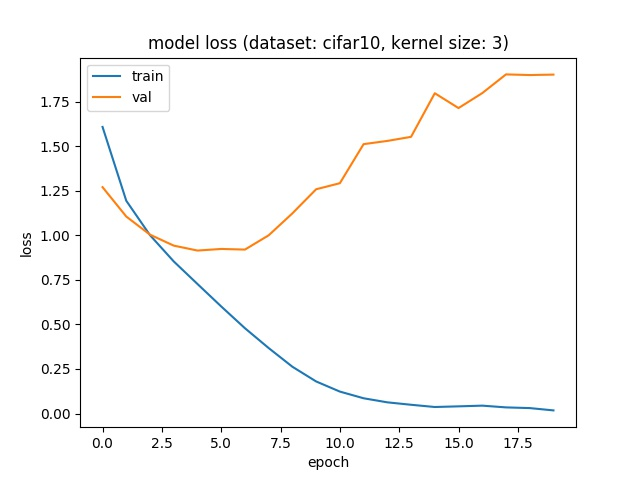
\includegraphics[width=0.3\columnwidth]{report_image/results/CIFAR10/cifar10_3_loss.jpg}  
}     
\subfigure[kernel size = 5] { 
\label{fig:b}     
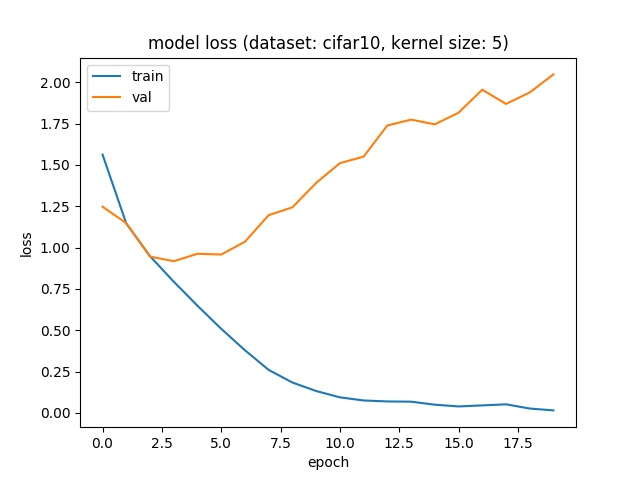
\includegraphics[width=0.3\columnwidth]{report_image/results/CIFAR10/cifar10_5_loss.jpg}     
}    
\subfigure[kernel size = 7] { 
\label{fig:c}     
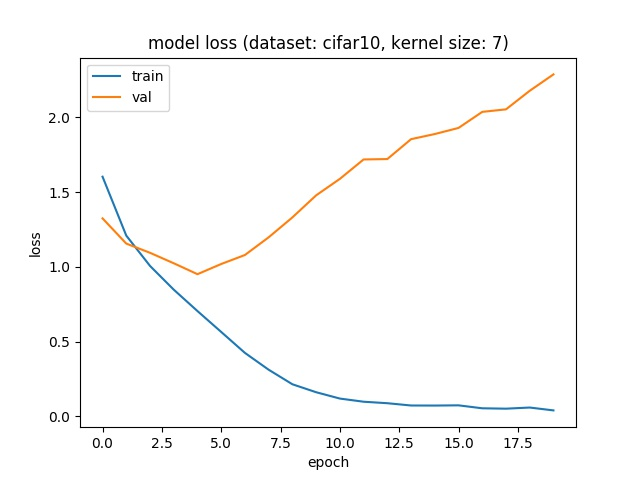
\includegraphics[width=0.3\columnwidth]{report_image/results/CIFAR10/cifar10_7_loss.jpg}     
}   
\subfigure[kernel size = 9] { 
\label{fig:d}     
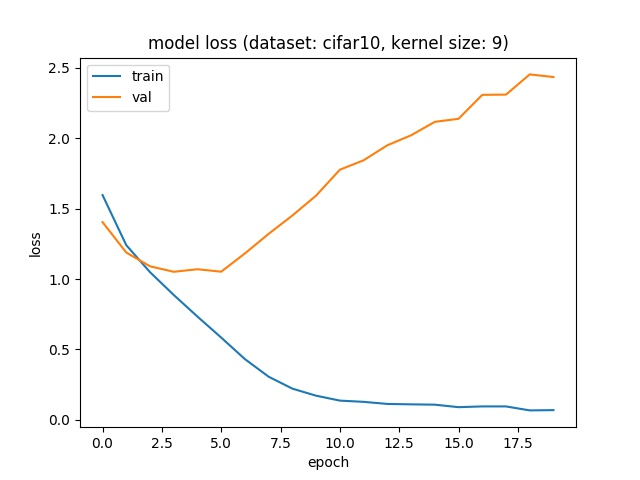
\includegraphics[width=0.3\columnwidth]{report_image/results/CIFAR10/cifar10_9_loss.jpg}     
}   
\subfigure[kernel size = 11] { 
\label{fig:e}     
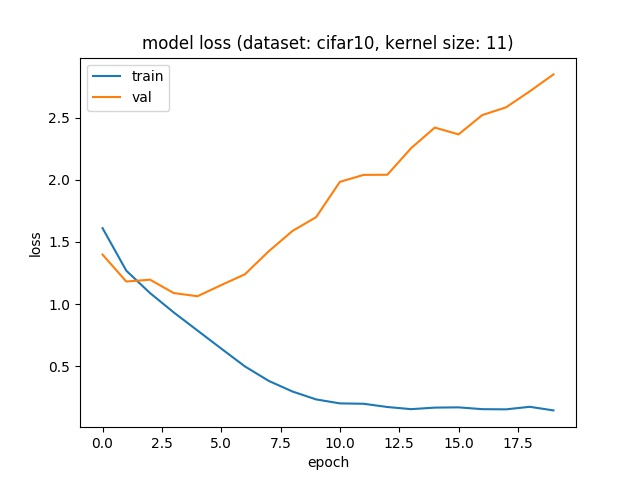
\includegraphics[width=0.3\columnwidth]{report_image/results/CIFAR10/cifar10_11_loss.jpg}     
}   
\caption{Loss with CIFAR-10}     
\label{Fig.cifar-10-loss}     
\end{figure}


We can see that all of CNNs with different kernel size have been overfitting. 

\subsection{17FLOWERS}

There are the several loss curves in Fig ~\ref{Fig.17flowers-loss} with using same CNN architecture but different convolutional kernel size.
\begin{figure}[htpb] \centering    
\subfigure[kernel size = 3] {
 \label{fig:a}     
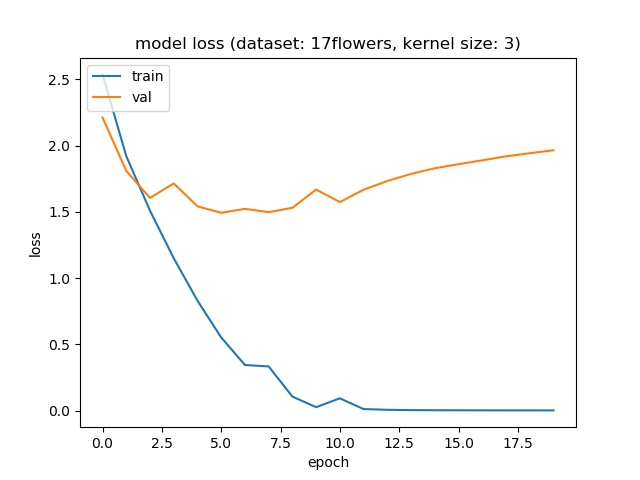
\includegraphics[width=0.3\columnwidth]{report_image/results/17FLOWERS/17flowers_3_loss.jpg}  
}     
\subfigure[kernel size = 5] { 
\label{fig:b}     
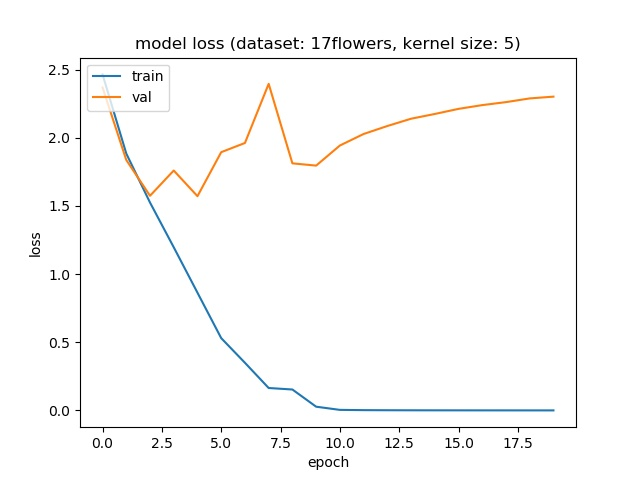
\includegraphics[width=0.3\columnwidth]{report_image/results/17FLOWERS/17flowers_5_loss.jpg}     
}    
\subfigure[kernel size = 7] { 
\label{fig:c}     
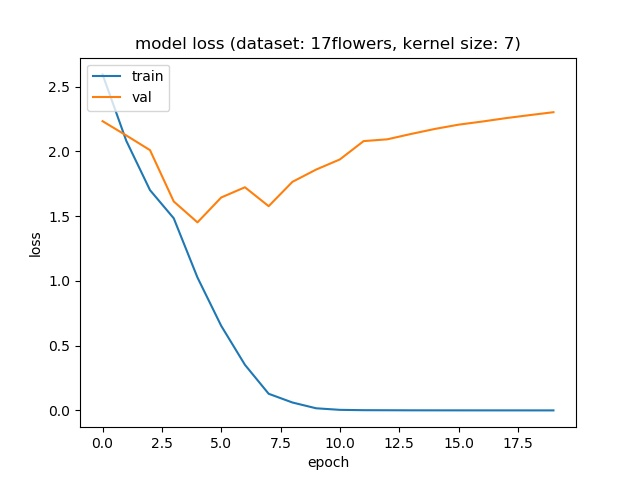
\includegraphics[width=0.3\columnwidth]{report_image/results/17FLOWERS/17flowers_7_loss.jpg}     
}   
\subfigure[kernel size = 9] { 
\label{fig:d}     
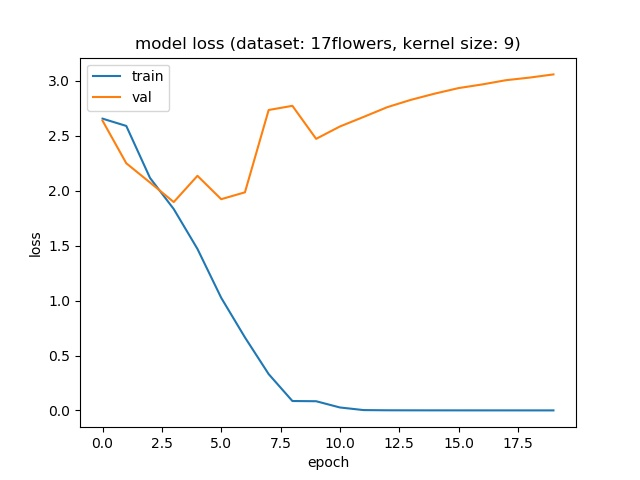
\includegraphics[width=0.3\columnwidth]{report_image/results/17FLOWERS/17flowers_9_loss.jpg}     
}   
\subfigure[kernel size = 11] { 
\label{fig:e}     
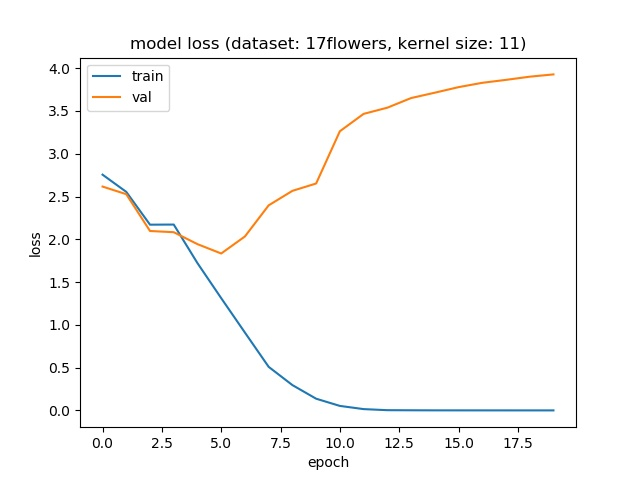
\includegraphics[width=0.3\columnwidth]{report_image/results/17FLOWERS/17flowers_11_loss.jpg}     
}   
\caption{Loss with 17FLOWERS}     
\label{Fig.17flowers-loss}     
\end{figure}


We can see that all of CNNs with different kernel size have been overfitting. 


\subsection{INDOOR67}

There are the several loss curves in Fig \ref{Fig.indoor67-loss} with using same CNN architecture but different convolutional kernel size.
\begin{figure}[htpb] \centering    
\subfigure[kernel size = 3] {
 \label{fig:a}     
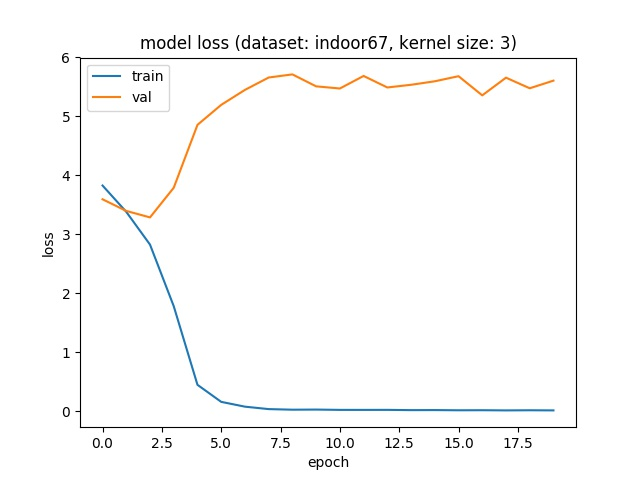
\includegraphics[width=0.3\columnwidth]{report_image/results/INDOOR67/indoor67_3_loss.jpg}  
}     
\subfigure[kernel size = 5] { 
\label{fig:b}     
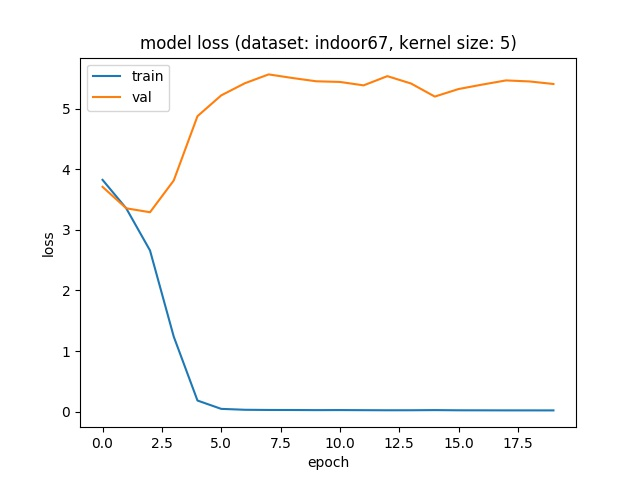
\includegraphics[width=0.3\columnwidth]{report_image/results/INDOOR67/indoor67_5_loss.jpg}     
}    
\subfigure[kernel size = 7] { 
\label{fig:c}     
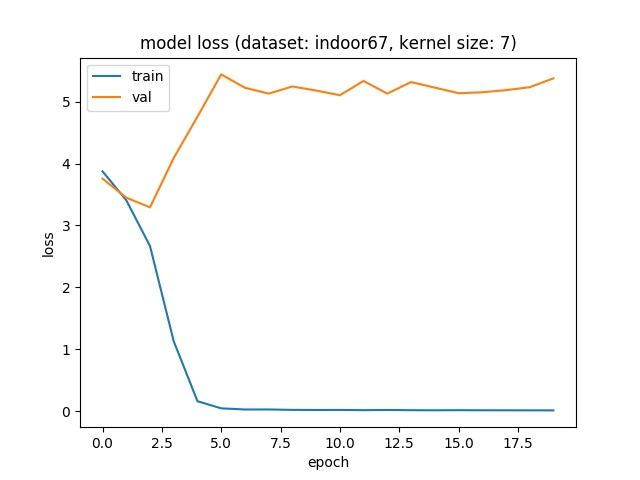
\includegraphics[width=0.3\columnwidth]{report_image/results/INDOOR67/indoor67_7_loss.jpg}     
}   
\subfigure[kernel size = 9] { 
\label{fig:d}     
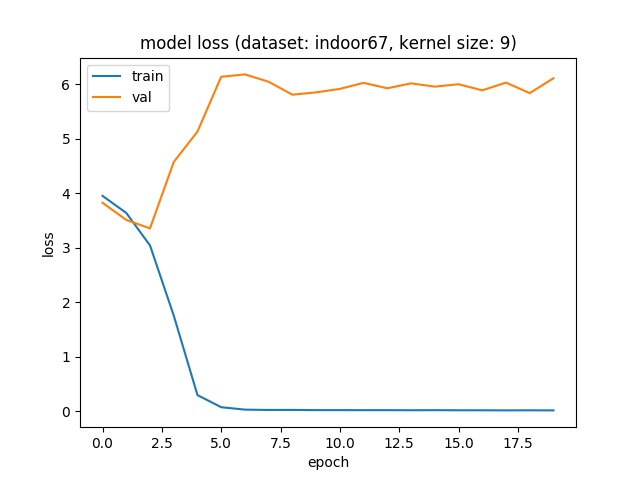
\includegraphics[width=0.3\columnwidth]{report_image/results/INDOOR67/indoor67_9_loss.jpg}     
}   
\subfigure[kernel size = 11] { 
\label{fig:e}     
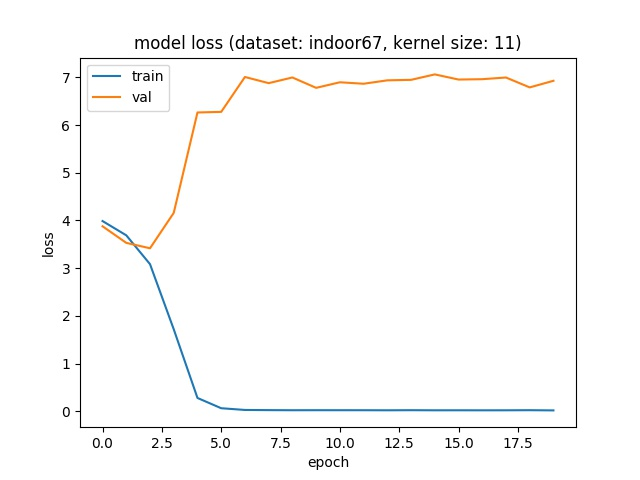
\includegraphics[width=0.3\columnwidth]{report_image/results/INDOOR67/indoor67_11_loss.jpg}     
}   
\caption{Loss with INDOOR67}     
\label{Fig.indoor67-loss}     
\end{figure}


We can see that all of CNNs with different kernel size have been overfitting. 

\subsection{TEXTURES}

There are the several loss curves in Fig ~\ref{Fig.textures-loss} with using same CNN architecture but different convolutional kernel size.
\begin{figure}[htpb] \centering    
\subfigure[kernel size = 3] {
 \label{fig:a}     
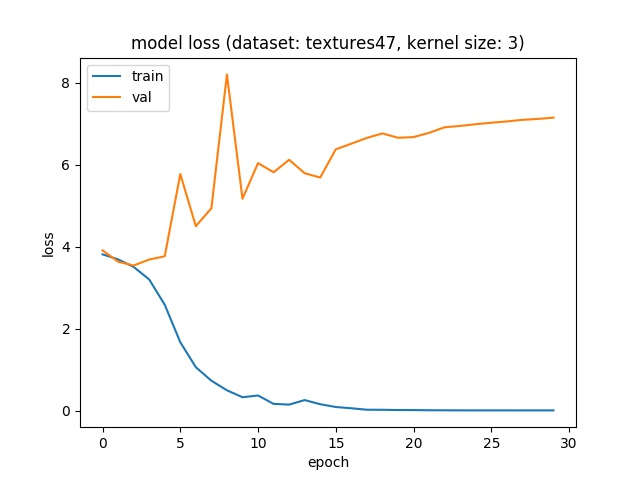
\includegraphics[width=0.3\columnwidth]{report_image/results/TEXTURES/textures47_3_loss.jpg}  
}     
\subfigure[kernel size = 5] { 
\label{fig:b}     
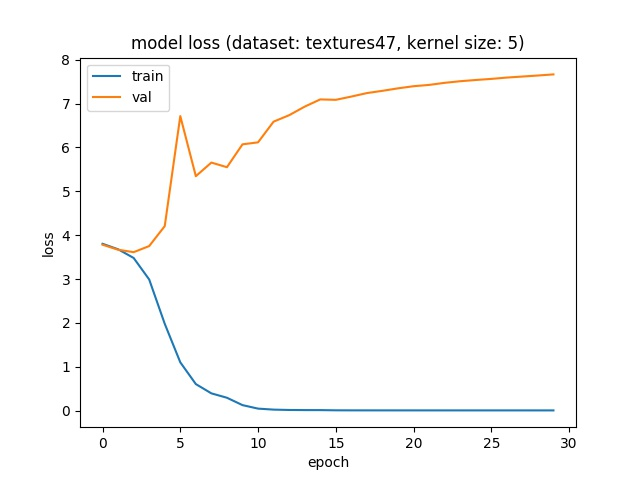
\includegraphics[width=0.3\columnwidth]{report_image/results/TEXTURES/textures47_5_loss.jpg}     
}    
\subfigure[kernel size = 7] { 
\label{fig:c}     
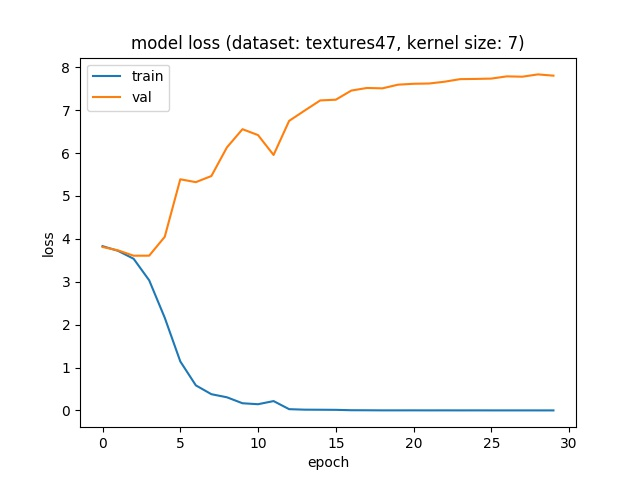
\includegraphics[width=0.3\columnwidth]{report_image/results/TEXTURES/textures47_7_loss.jpg}     
}   
\subfigure[kernel size = 9] { 
\label{fig:d}     
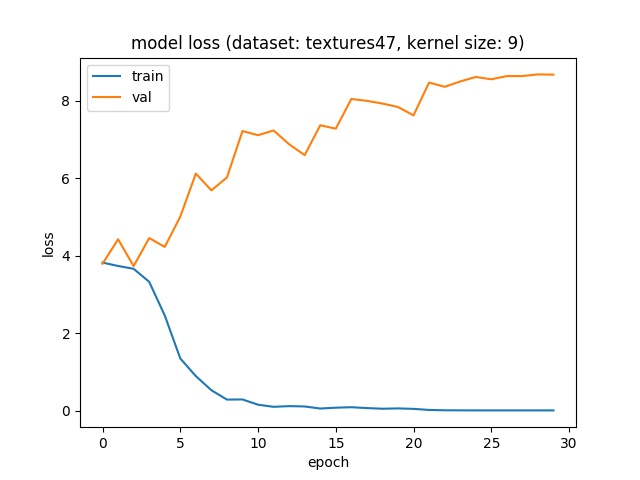
\includegraphics[width=0.3\columnwidth]{report_image/results/TEXTURES/textures47_9_loss.jpg}     
}   
\subfigure[kernel size = 11] { 
\label{fig:e}     
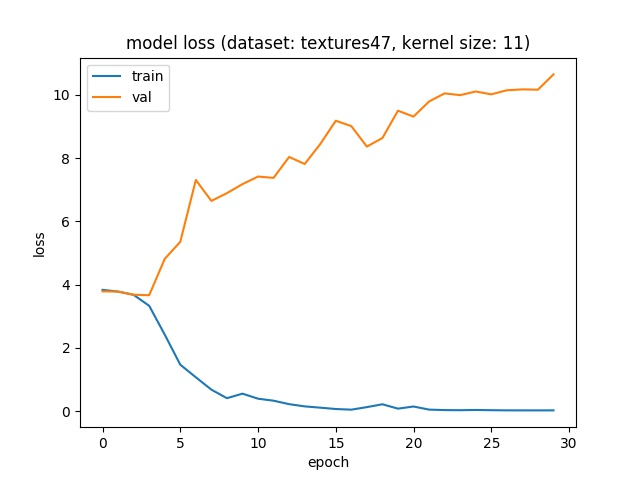
\includegraphics[width=0.3\columnwidth]{report_image/results/TEXTURES/textures47_11_loss.jpg}     
}   
\caption{Loss with TEXTURES}     
\label{Fig.textures-loss}     
\end{figure}


We can see that all of CNNs with different kernel size have been overfitting. 

\section{Discussion}

I selected the minimum loss from every loss figure to denote the best effect of CNN with these kernel size. The minimum loss with different kernel size is drawn in Fig ~\ref{Fig.minimum-loss}:

\begin{figure}[htpb] \centering    
\subfigure[CIFAR-10] {
 \label{fig:a}     
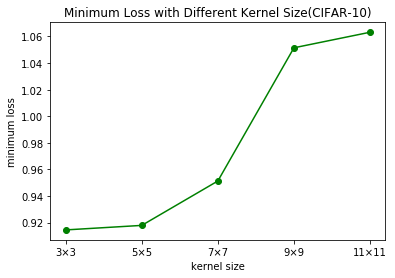
\includegraphics[width=0.45\columnwidth]{report_image/results/cifar10_minimum_loss.png}  
}     
\subfigure[17FLOWERS] { 
\label{fig:b}     
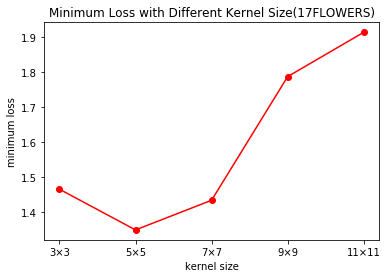
\includegraphics[width=0.45\columnwidth]{report_image/results/17flowers_minimum_loss.png}     
}    
\subfigure[INDOOR67] { 
\label{fig:c}     
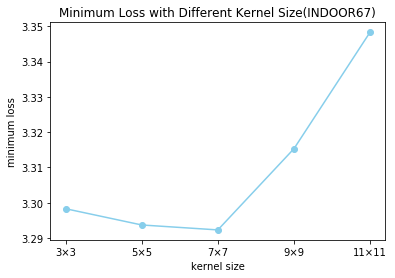
\includegraphics[width=0.45\columnwidth]{report_image/results/indoor67_minimum_loss.png}     
}   
\subfigure[TEXUTURES] { 
\label{fig:d}     
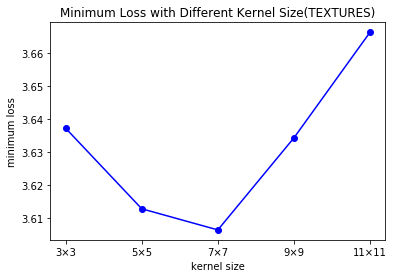
\includegraphics[width=0.45\columnwidth]{report_image/results/textures_minimum_loss.png}     
}   
\caption{minimum loss with different kernel size}     
\label{Fig.minimum-loss}     
\end{figure}

In the CIFAR-10 figure, the loss increases from 0.9145 to 1.0632 with kernel size increasing. When kernel size of convolutional layer is equal to 3(or $3\times3$), CNN has a minimum loss that I called optimum kernel size. When we focus on 17FLOWERS figure, there is a little different from CIFAR-10 because optimum kernel size is 5(or $5\times5$) but not 3(or $3\times3$). Then looking at INDOOR67, its optimum kernel size is up to 7(or $7\times7$), same as the TEXTURES dataset.


From the above phenomenon, we can draw conclusions that different dataset has different optimum kernel size though their CNN architecture are same. I have some explainations for the phenomenon as follows:

   \begin{itemize}
      \item  \textbf{regularization}: bigger kernel size means more weights and the CNN model will become more complex. In the report, all of these CNN models with different datasets and kernel sizes are have been trained to overfitting. So according to Occam's rezor, smaller kernel size will increase the model generation. That is to say smaller kernel size can make contributions to reduce validation loss.
      \item  \textbf{category of dataset}:  We can distinguish the class of images in CIFAR-10 easily. But it may be a little difficult to identifying the category of pictures in TEXTURES dataset. When the category of dataset is widely distributed like CIFAR-10 from horse to airplane, small kernel size is enough to capture infromation from dataset. If the classes between dataset are very closed each other, we need bigger kernel size to extract more information to recognize them. 
   \end{itemize}


On the one hand, bigger kernel size will increase model complexity leading to higher validation loss. On the other hand, bigger kernel size can capture more information from dataset especially for the datasets which categories are very closed so that the validation loss could be reduced. Optimum kernel size for a specific dataset should achieve balance between the two.



\section{Conclusions}
In the report, I do some research on the convolutional kernel size. There is a connection between optimum kernel size and different datasets for same CNN architecture. Small kernel size cannot extract enough information but bigger kernel size will increase model comlexity. We need to balance them to find optimum kernel size.

\newpage

\renewcommand\refname{Reference}
\bibliographystyle{plain}
\bibliography{ref}

\end{document}
